\chapter{Testes}
\label{cha:Testes}

Afim de satisfazer todos os requisitos descritos no capítulo \ref{cha:Requisitos}, foram efetuados testes do sistema e algoritmo durante toda a fase de desenvolvimento. Esses testes eram efetuados de maneira não estruturada, apenas para testar todos os possíveis casos de erro. Foi considerada a metodologia de \textit{Desenvolvimento orientado a testes}, que planeja o desenvolvimento primeiro de testes unitários e de integração, para depois o desenvolvimento da aplicação em si. Porém, a implantação dessa metodologia costuma aumentar consideravelmente o tempo de desenvolvimento de aplicações, por isso ela não foi implementada.

Para verificar os requisitos RF01-06, foi testado se o algoritmo recebia todos os parâmetros necessários, e se retornava adequadamente quando os parâmetros não eram satisfeitos. Como a implementação do algoritmo é um modelo matemático, pode-se observar que o requisito RNF2 (que determina que o algoritmo deve retornas os mesmos resultados para as mesmas entradas) foi atendido com sucesso.

Foram efetuados testes de performance, para verificar se os requisitos RNF1 e RNF3 foram satisfeitos. A figura \ref{fig:teste-performance} representa um teste de performance, com 40 usuários simultâneos autenticados solicitando recomendações diferentes a cada 1-5 segundos. É possível observar que o tempo médio de resposta das recomendações foi 20 milisegundos, e não houve nenhuma falha no sistema ou algoritmo. O teste de performance foi desenvolvido usando o framework \textit{Locust} \cite{site-locust}, utilizando a linguagem Python.

\begin{figure}[ht]
    \begin{center}
    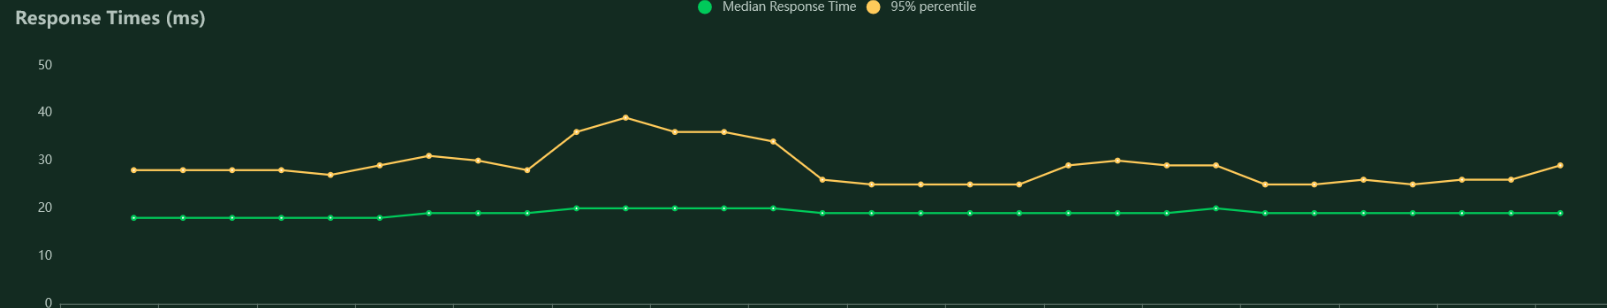
\includegraphics[width=390pt]{figuras/teste-performance.png}
    \caption{Teste de performance da recomendação}
    \label{fig:teste-performance}
    \end{center}
\end{figure}

Ao ter-se uma versão com todas os requisitos atendidos, o processo de testes com os usuários deu-se inicío. A metodologia dos testes foi:

\begin{enumerate}
    \item Apresentar a ideia do sistema e do algoritmo de recomendação;
    \item Apresentar todas as possíveis funcionalidades do sistema;
    \item Criar uma grade horária como exemplo, utilizando-se de todas as funcionalidades do sistema;
    \item Permitir que o usuário faça sua autenticação e crie um grade horária;
    \item Ouvir o feedback do usuário.
\end{enumerate}

O processo de testes com os usuários não foi um simples. Apesar de o sistema possuir todas as suas funcionalidades, o design e as interações ainda estavam incompletas, o que dificultava o entendimento do usuário quanto às funcionalidades. Nem todas as possibilidades estavam bem descritas, e só foram compreendidas por completo após explicações detalhadas.

Os resultados dos testes estão descritos no capítulo \ref{cha:Uso real}.